\documentclass{article}
\linespread{1.3}
\usepackage[margin=50pt]{geometry}
\usepackage{amsmath, amsthm, amssymb, amsthm, tikz, fancyhdr, graphicx, subfig}
\pagestyle{fancy}
\renewcommand{\headrulewidth}{0pt}
\newcommand{\changefont}{\fontsize{15}{15}\selectfont}

\newcommand{\field}[1]{\mathbb{#1}}
\newcommand{\1}{\mathbf{1}}
\newcommand{\E}{\mathbb{E}} 
\renewcommand{\P}{\mathbb{P}}
\newcommand{\R}{\field{R}} % real domain
% \newcommand{\C}{\field{C}} % complex domain
\newcommand{\F}{\field{F}} % functional domain

\newcommand{\T}{^{\textrm T}} % transpose

\def\diag{\text{diag}}

%% operator in linear algebra, functional analysis
\newcommand{\inner}[2]{#1\cdot #2}
\newcommand{\norm}[1]{\left\|#1\right\|}
\newcommand{\twonorm}[1]{\|#1\|_2^2}
% operator in functios, maps such as M: domain1 --> domain 2
\newcommand{\Map}[1]{\mathcal{#1}}
\renewcommand{\theenumi}{\alph{enumi}} 

\newcommand{\Perp}{\perp \! \! \! \perp}

\newcommand\independent{\protect\mathpalette{\protect\independenT}{\perp}}
\def\independenT#1#2{\mathrel{\rlap{$#1#2$}\mkern2mu{#1#2}}}
\newcommand{\vct}[1]{\boldsymbol{#1}} % vector
\newcommand{\mat}[1]{\boldsymbol{#1}} % matrix
\newcommand{\cst}[1]{\mathsf{#1}} % constant
\newcommand{\ProbOpr}[1]{\mathbb{#1}}
\newcommand{\points}[1]{\small\textcolor{magenta}{\emph{[#1 points]}} \normalsize}
\date{{}}

\fancypagestyle{firstpageheader}
{
  \fancyhead[R]{\changefont Michael Huang \\ CSE 446 \\ Homework 3}
}

\begin{document}

\thispagestyle{firstpageheader}

\section*{Collaborators}
{\Large 
Jimmy Guo, Neil Kagalwala, Andrew Wang
}
\section*{A.1}
{\Large 

\subsection*{a.}

If the RBF kernel underfits the training set, we should decrease the bandwidth $\sigma$. Underfitting indicates a smoother fit and lower variance, so we want to decrease $\sigma$ so that we fit the training points more tightly.
% more narrow bumps and fits data more tightly

\subsection*{b.}

True. With a non-convex loss function, gradient descent is not guaranteed to go all the way towards the global minimum, and could even stagnate or increase.
% Could increase?

\subsection*{c.}

False. When training a deep neural network, we should initialize weights to random values. One reason for this is that with any equal weight initialization, all nodes will have the same gradient, so the nodes will end up all following the same pattern and an ineffective model overall.

\subsection*{d.}

True. We try to use non-linear activation functions in order to introduce non-linearity into the network. If we only had linear activation functions, then the model would essentially just output a linear function, since no matter how many layers, all the linear functions would naturally sum together, and lead to what is essentially basic logistic regression.

\subsection*{e.}

True. The time complexity for the forward pass is lower than that of the backward pass in the backpropagation algorithm. backpropagation first requires calculating values via forward-propagation itself, and then performing error calculation and gradient descent to update these values.

}

\section*{A.2}
{\Large

We aim to show that $K(x, x') = e^{-\frac{(x-x')^2}{2}}$ is a kernel function for the defined feature map, or that $\phi (x) \cdot \phi (x') = e^{-\frac{(x-x')^2}{2}}$. \\ \\
We are given that the $i$th component of the vector $\phi(x)$ is defined as $\frac{1}{\sqrt{i!}} e^{-x^2/2} x^i$, and we can naturally express $\phi(x')$ as  $\frac{1}{\sqrt{i!}} e^{-(x')^2 / 2} (x')^i$.
% $= \sqrt{\frac{e^{-x^2}}{i}} x^i$
\\
In multiplying $\phi(x) \cdot \phi(x')$, we have that we are essentially multiplying the elements of each column against each other, that is, $\phi(x) \cdot \phi(x')$ \\
$= \sum_{i=0}^{n} \text{element}_i \text{ of } \phi(x) \cdot \text{element}_i \text{ of } \phi(x')$ \\
$= \sum_{i=0}^{n} \frac{1}{\sqrt{i!}} e^{-x^2/2} x^i \cdot \frac{1}{\sqrt{i!}} e^{-(x')^2 / 2} (x')^i$ \\
$= \sum_{i=0}^{n} \frac{1}{i!} e^{-x^2/2} x^i \cdot e^{-(x')^2 / 2} (x')^i$ \\
$= \sum_{i=0}^{n} \frac{1}{i!} e^{-x^2/2 - (x')^2 / 2} x^i (x')^i$ \\
$= e^{-x^2/2 - (x')^2 / 2} \cdot \sum_{i=0}^{n} \frac{1}{i!} (xx')^i$ \\ \\
% maybe change the n to \infty
We know that the Taylor series expansion of $z \mapsto e^z$ is $\sum_{i=0}^{\infty} \frac{z^i}{i!}$ to simplify the second term of the product, as we know that $\phi(x)$ is a vector of infinite length: \\
$= e^{-x^2/2 - (x')^2 / 2} \cdot e^{(xx')}$ \\
$= e^{-x^2/2 - (x')^2 / 2 + (xx')} $ \\
$= e^{\frac{-x^2 - (x')^2 + 2xx'}{2}} $ \\
$= e^{\frac{-(x^2 + (x')^2 - 2xx')}{2}} $ \\
$= e^{\frac{-(x - x')^2)}{2}} $ \\
which is exactly what we sought to show.

}

\newpage
\section*{A.3}

{\Large 

\subsection*{a.}

\textbf{poly:} \\
$d: 18.0$ \\
$\lambda: 10^{-5}$ \\ 
\textbf{rbf:} \\
$\gamma: 30$ \\
$\lambda: 10^{-1}$

\subsection*{b.}

\begin{figure}[h]
  \centering
  \subfloat[poly true vs predict]{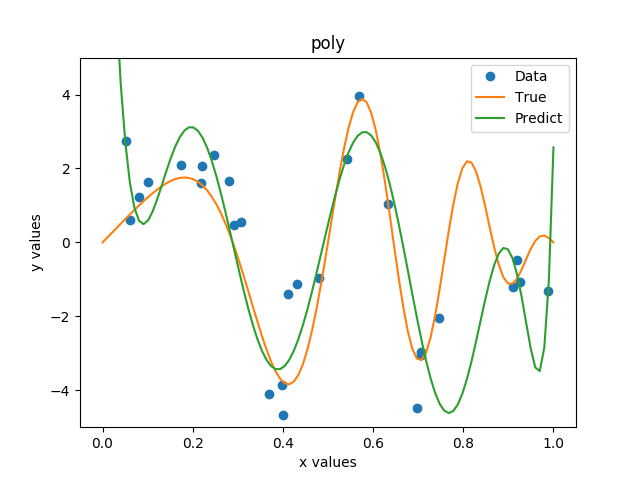
\includegraphics[width=100mm]{../hw3-code/results/a3_bi.png}}
  \subfloat[rbf true vs predict]{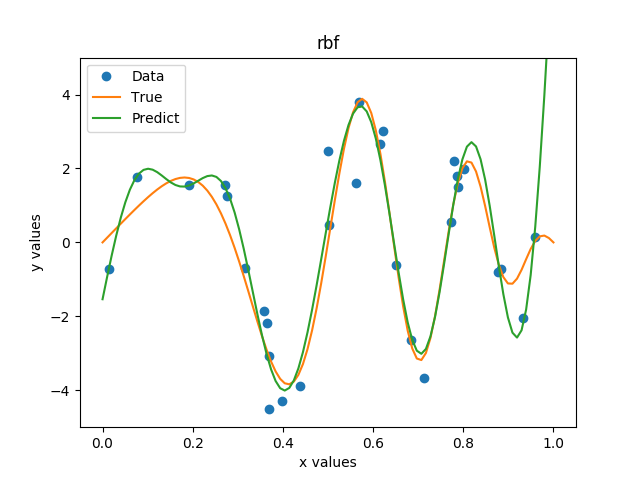
\includegraphics[width=100mm]{../hw3-code/results/a3_bii.png}}
\end{figure}

\newpage

\subsection*{c.}

\begin{figure}[h]
  \centering
  \subfloat[poly with confidence intervals]{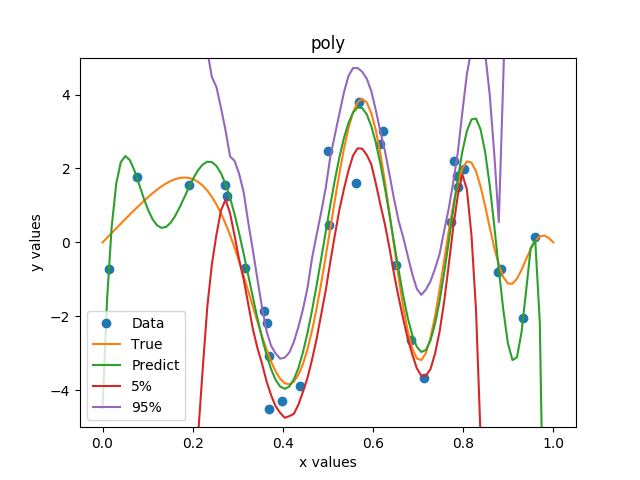
\includegraphics[width=100mm]{../hw3-code/results/a3_ci.png}}
  \subfloat[rbf with confidence intervals]{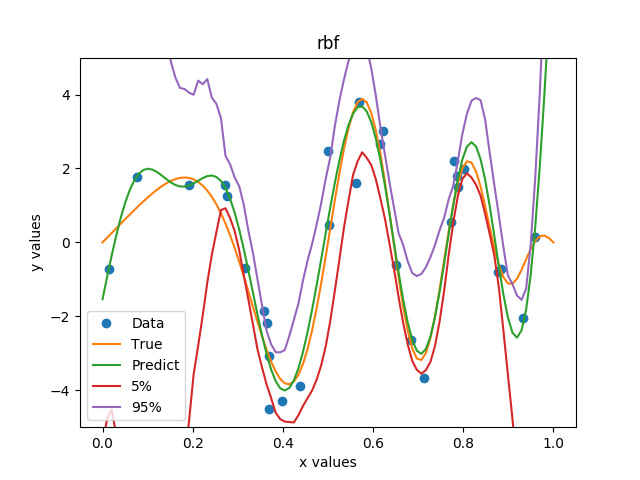
\includegraphics[width=100mm]{../hw3-code/results/a3_cii.png}}
\end{figure}

\subsection*{d.}
\begin{figure}[h]
  \centering
  \subfloat[poly true vs predict]{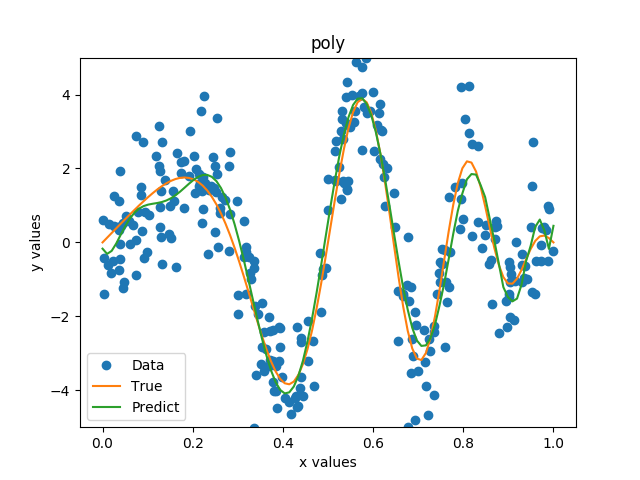
\includegraphics[width=100mm]{../hw3-code/results/a3_d.bi.png}}
  \subfloat[rbf true vs predict]{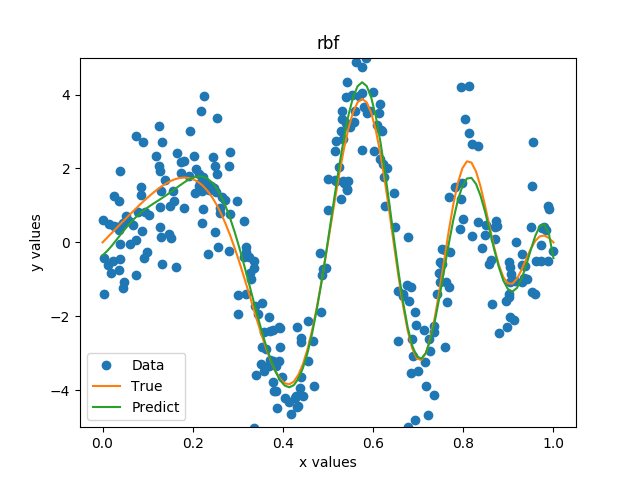
\includegraphics[width=100mm]{../hw3-code/results/a3_d.bii.png}}
\end{figure}
\begin{figure}[h]
  \centering
  \subfloat[poly with confidence intervals]{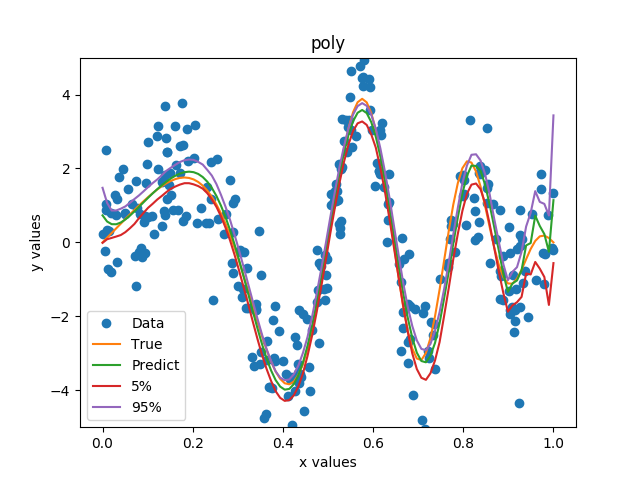
\includegraphics[width=100mm]{../hw3-code/results/a3_d.ci.png}}
  \subfloat[rbf with confidence intervals]{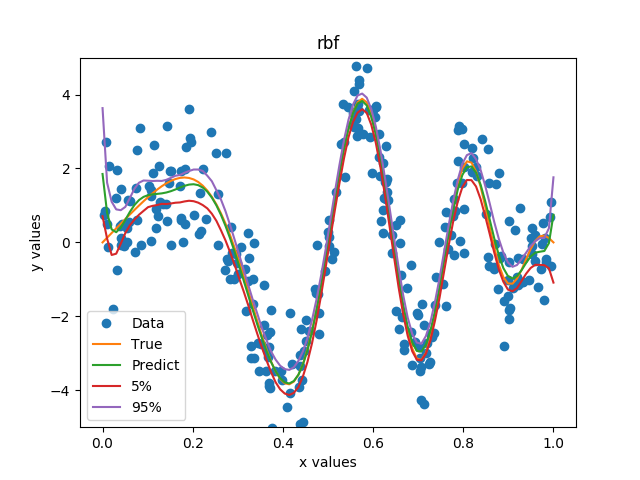
\includegraphics[width=100mm]{../hw3-code/results/a3_d.cii.png}}
\end{figure} 
\newpage
\textbf{poly:} \\
$d: 22.0$ \\
$\lambda: 10^{-7}$ \\ 
\textbf{rbf:} \\
$\gamma: 24.0$ \\
$\lambda: 10^{-4}$

\subsection*{e.}

For this problem, use the $\widehat{f}_{\rm poly}(x)$ and $\widehat{f}_{\rm rbf}(x)$ learned in part d. Suppose $m=1000$ additional samples $(x_1',y_1'),\dots,(x_m',y_m')$ are drawn i.i.d. the same way the first $n$ samples were drawn. 
  
  \medskip
  
  Use the non-parametric bootstrap with $B=300$ to construct a confidence interval on
  \[
    \E\left[ \left(Y-\widehat{f}_{\rm poly}(X)\right)^2 - \left(Y-\widehat{f}_{\rm rbf}(X)\right)^2 \right]
  \]
  (i.e. randomly draw with replacement $m$ samples denoted as $\{(\widetilde{x}_i',\widetilde{y}_i')\}_{i=1}^m$ from $\{(x_i',y_i')\}_{i=1}^m$ and compute $\frac{1}{m} \sum\limits_{i=1}^m \left[ \left(\widetilde{y}_i'-\widehat{f}_{\rm poly}(\widetilde{x}_i')\right)^2 - \left(\widetilde{y}_i'-\widehat{f}_{\rm rbf}(\widetilde{x}_i')\right)^2 \right]$, repeat this $B$ times) and find $5\%$ and $95\%$ percentiles. Report these values.
  
  \medskip
  
  Using this confidence interval, is there statistically significant evidence to suggest that one of $\widehat{f}_{\rm rbf}$ and $\widehat{f}_{\rm poly}$ is better than the other at predicting $Y$ from $X$? (Hint: does the confidence interval contain $0$?)

}

\section*{A.4}
{\Large 

\begin{figure}[h]
  \centering
  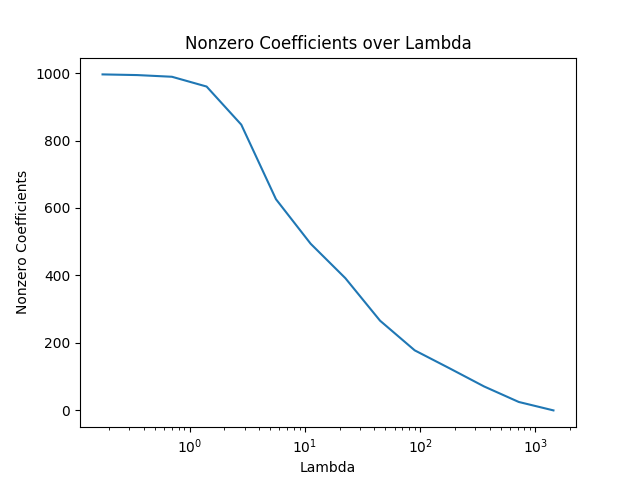
\includegraphics[width=120mm]{../hw2-code/results/a4_a.png}
\end{figure}

\subsection*{a.}

Let $W_0 \in \mathbb{R}^{h \times d}$, $b_0 \in \mathbb{R}^h$, $W_1 \in \mathbb{R}^{k \times h}$, $b_1 \in \mathbb{R}^k$ and $\sigma(z)\colon \mathbb{R} \to \mathbb{R}$
some non-linear activation function applied element-wise. Given some $x \in \mathbb{R}^{d}$, the forward pass of the wide, shallow network can be formulated as:

\[
    \mathcal{F}_1(x) := W_1 \sigma(W_0 x + b_0) + b_1
\]


Use $h=64$ for the number of hidden units and choose an appropriate learning rate.
Train the network until it reaches $99\%$ accuracy on the training data and provide a training plot (loss vs. epoch).
Finally evaluate the model on the test data and report both the accuracy and the loss.

\subsection*{b.}

Let $W_0 \in \mathbb{R}^{h_0 \times d}$, $b_0 \in \mathbb{R}^{h_0}$, $W_1 \in \mathbb{R}^{h_1 \times h_0}$, $b_1 \in \mathbb{R}^{h_1}$,
$W_2 \in \mathbb{R}^{k \times h_1}$, $b_2 \in \mathbb{R}^{k}$ and $\sigma(z) : \mathbb{R} \rightarrow \mathbb{R}$
some non-linear activation function. Given some $x \in \mathbb{R}^{d}$, the forward pass of the network can be formulated as:

\[
    \mathcal{F}_2(x) := W_2 \sigma(W_1 \sigma(W_0 x + b_0) + b_1) + b_2
\]

Use $h_0 = h_1 = 32$ and perform the same steps as in part a.

\subsection*{c.}

Compute the total number of parameters of each network and report them. Then compare the number of parameters as well as the test accuracies the networks achieved. Is one of the approaches (wide, shallow vs. narrow, deeper) better than the other? Give
an intuition for why or why not.

\textbf{Wide + shallow} \\ \\
Number of parameters: $784 \cdot 64 + 64 \cdot 1 + 64 \cdot 10 + 10 \cdot 1 = 50176 + 64 + 640 + 10 = 50890$  \\
Test accuracy: \\ \\
\textbf{Narrow + deeper} \\ \\
Number of parameters: $784 \cdot 32 + 32 \cdot 1 + 32 \cdot 32 + 32 + 32 \cdot 10 + 10 = 25088 + 32 + 1024 + 32 + 320 + 10 = 26506$  \\
Test accuracy: \\ \\
Narrow and deeper should be better. Generalizing vs memorizing.

}

\section*{A.5}
{\Large 

\begin{figure}[h]
  \centering
  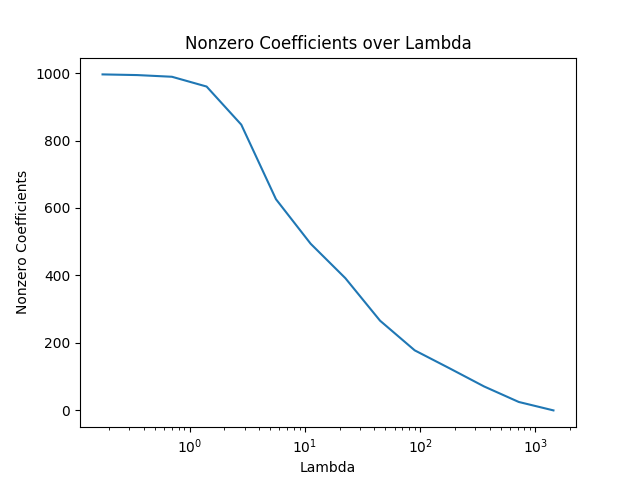
\includegraphics[width=120mm]{../hw2-code/results/a4_a.png}
\end{figure}

\framebox[1.1\width]{\textbf{Applicable output can be found in a5.txt, which I did not paste in due to its length}}

So far we have trained very small neural networks from scratch. As mentioned in the previous problem, modern neural networks are much larger and more difficult to train and validate. In practice, it is rare to train such large networks from scratch. This is because it is difficult to obtain both the massive datasets and the computational resources required to train such networks. \\
 
 Instead of training a network from scratch, in this problem, we will use a network that has already been trained on a very large dataset (ImageNet) and adjust it for the task at hand. This process of adapting weights in a model trained for another task is known as \textit{transfer learning}.
\begin{itemize}
    \item Begin with the pretrained \text{AlexNet} model from \texttt{torchvision.models} for both tasks below. \text{AlexNet} achieved an early breakthrough performance on \texttt{ImageNet} and was instrumental in sparking the deep learning revolution in 2012.
    \item Do not modify any module within AlexNet that is not the final classifier layer.
    \item The output of AlexNet comes from the $6$-th layer of the classifier. Specifically, \texttt{model.classifer[6] = nn.Linear(4096, 1000)}. To use AlexNet with CIFAR-10, we will reinitialize (replace) this layer with \texttt{nn.Linear(4096, 10)}. This re-initializes the weights, and changes the output shape to reflect the desired number of target classes in CIFAR-10. 
\end{itemize}

\subsection*{a.}

\textbf{Use AlexNet as a fixed feature extractor:} Add a new linear layer to replace the existing classification layer, and only adjust the weights of this new layer (keeping the weights of all other layers fixed). Provide plots for training loss and validation loss over the number of epochs. Report the highest validation accuracy achieved. Finally, evaluate the model on the test data and report both the accuracy and the loss.  
    
    When using AlexNet as a fixed feature extractor, make sure to freeze all of the parameters in the network \textit{before} adding your new linear layer:
    \begin{verbatim}
    model = torchvision.models.alexnet(pretrained=True)
    for param in model.parameters():
        param.requires_grad = False
    model.classifier[6] = nn.Linear(4096, 10)
    \end{verbatim}

\subsection*{b.}

\textbf{Fine-Tuning:} The second approach to transfer learning is to fine-tune the weights of the pre-trained network, in addition to training the new classification layer. In this approach, all network weights are updated at every training iteration; we simply use the existing AlexNet weights as the ``initialization'' for our network (except for the weights in the new classification layer, which will be initialized using whichever method is specified in the constructor) prior to training on CIFAR-10. Following the same procedure, report all the same metrics and plots as in the previous question. 

}

\section*{A.6}
{\Large 

\begin{figure}[h]
  \centering
  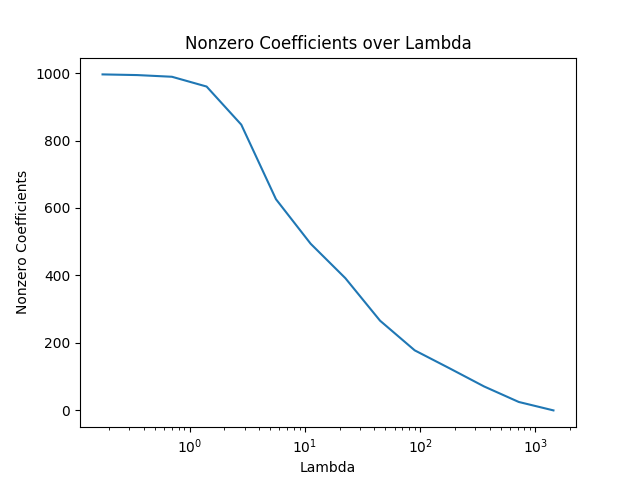
\includegraphics[width=120mm]{../hw2-code/results/a4_a.png}
\end{figure}

\framebox[1.1\width]{\textbf{Applicable output can be found in a6a.txt / a6b.txt / a6c.txt / a6d.txt, which I did not paste in due to its length}}

\subsection*{a.}

\textbf{Fully-connected output, 0 hidden layers (logistic regression):} this network has no hidden layers and linearly maps the input layer to the output layer. This can be written as 
  \begin{align*}
    x^{\rm out} &= W (x^{\rm in}) +b
  \end{align*} 
  
  where $x^{\rm out} \in \R^{10}$, $x^{\rm in} \in \R^{32 \times 32 \times 3}$, $W \in \R^{10 \times 3072}$, $b \in \R^{10}$ since $3072 = 32 \cdot 32 \cdot 3$. For a tensor $x \in \R^{a \times b \times c}$, we let $(x) \in \R^{a b c}$ be the reshaped form of the tensor into a vector (in an arbitrary but consistent pattern).

\subsection*{b.}

\textbf{Fully-connected output, 1 fully-connected hidden layer:} this network has one hidden layer denoted as $x^{\rm hidden} \in \R^{M}$ where $M$ will be a hyperparameter you choose ($M$ could be in the hundreds). The non-linearity applied to the hidden layer will be the \texttt{relu} ($\mathrm{relu}(x) = \max\{0,x\}$. This network can be written as
  \begin{align*}
    x^{\rm out} &= W_2 \mathrm{relu}(W_1 (x^{\rm in}) +b_1) + b_2
  \end{align*}
  where $W_1 \in \R^{M \times 3072}$, $b_1 \in \R^M$, $W_2 \in \R^{10 \times M}$, $b_2 \in \R^{10}$.

\subsection*{c.}

\textbf{Convolutional layer with max-pool and fully-connected output:} for a convolutional layer $W_1$ with filters of size $k \times k \times 3$, and $M$ filters (reasonable choices are $M=100$, $k=5$), we have that $\mathrm{Conv2d}(x^{\rm in}, W_1) \in \R^{(33-k) \times (33-k) \times M}$.
  
\begin{itemize}
    \item Each convolution will have its own offset applied to each of the output pixels of the convolution; we denote this as $\mathrm{Conv2d}(x^{\rm in}, W) + b_1$ where $b_1$ is parameterized in $\R^M$. Apply a \texttt{relu} activation to the result of the convolutional layer. 
    \item Next, use a max-pool of size $N \times N$ (a reasonable choice is $N=14$ to pool to $2 \times 2$ with $k=5$) we have that $\textrm{MaxPool}( \mathrm{relu}( \mathrm{Conv2d}(x^{\rm in}, W_1)+b_1)) \in \R^{\lfloor\frac{33-k}{N}\rfloor \times \lfloor\frac{33-k}{N}\rfloor \times M}$.
    \item We will then apply a fully-connected layer to the output to get a final network given as
        \begin{align*}
        x^{\rm output} = W_2 (\textrm{MaxPool}( \mathrm{relu}( \mathrm{Conv2d}(x^{\rm input}, W_1)+b_1))) + b_2
        \end{align*}
  where $W_2 \in \R^{10 \times M (\lfloor\frac{33-k}{N}\rfloor)^2}$, $b_2 \in \R^{10}$.
\end{itemize}

The parameters $M,k,N$ (in addition to the step size and momentum) are all hyperparameters, but you can choose a reasonable value. Tuning can be performed (optionally) in the next subproblem.

\subsection*{d.}

\textbf{Tuning:} Return to the original network you were left with at the end of the tutorial \emph{Training a classifier}. Tune the different hyperparameters (number of convolutional filters, filter sizes, dimensionality of the fully-connected layers, stepsize, etc.) and train for a sufficient number of iterations to achieve a \emph{test accuracy} of at least 70\%. Provide the hyperparameter configuration used to achieve this performance.


}

\section*{}
{\Large 
\newpage

\begin{verbatim}
  # helpers.py
# Applicable helpers for HW3

import numpy as np
import matplotlib.pyplot as plt

import constants as c

def generate_data(n):
  print("generating data")

  f_star = lambda x: 4 * np.sin(np.pi * x) * np.cos(6 * np.pi * x ** 2)

  X = np.random.uniform(0, 1, (n, ))
  error = np.random.normal(0, 1, (n, ))
  Y = f_star(X) + error

  return X, Y, f_star

def ylimit_plot(bot, top):
  plt.ylim(bot, top)

def plot_multiple(title, file_name, x, y, data_list, label_list, ylimits=None):
  print("plotting og, true, and fit")

  plt.plot(x, y, "o")
  
  for data_set in data_list:
    plt.plot(c.x_list, data_set)

  if ylimits is not None:
    ylimit_plot(ylimits[0], ylimits[1])

  plt.title(title)
  plt.xlabel("x values")
  plt.ylabel("y values")
  plt.legend(label_list)

  plt.savefig(c.results_path + file_name + c.png_exten)
  plt.close()

def plot_acc(dataset, legends, filename, set_type, epochs=12):
  
  epoch_list = list(range(1, epochs + 1))
  
  for item in dataset:
    plt.plot(epoch_list, item)

  plt.title(set_type + " accuracy over time")
  plt.xlabel("epochs")
  plt.ylabel("accuracy")
  
  plt.legend(legends)

  plt.savefig(filename)
\end{verbatim}

\begin{verbatim}
# constants.py
# Applicable constants for HW3

import numpy as np
import os

home_dir_path = os.path.dirname(os.path.dirname(os.path.abspath(__file__)))

data_path = home_dir_path + '/data/'
results_path = home_dir_path + '/results/'

png_exten = '.png'

hp_list = list(np.linspace(1, 30, 30))
lamb_list = [10 ** -x for x in np.linspace(0, 10, 11)]

pred_labels = ['Data', 'True', 'Predict']
pct_labels = ['Data', 'True', 'Predict', '5%', '95%']
x_list = list(np.linspace(0, 1, 100))

a3b_ylimits = [-5, 5]
num_fold = 10
B = 300
m = 1000
\end{verbatim}
}

\end{document}